\documentclass[11pt]{article}
\usepackage[paperwidth=8.5in,paperheight=11in,margin=1.25in]{geometry}
\usepackage[strict]{changepage}
\usepackage{booktabs, threeparttable, adjustbox, tabularx, longtable}
\usepackage{amsmath, amssymb, amsthm, bbm}
\usepackage{hyperref, achicago}
\usepackage{caption, graphicx}
\usepackage{secdot, sectsty}
\usepackage{pdflscape}
\usepackage{placeins}
\usepackage{setspace}
\usepackage{xcolor}

\allsectionsfont{\rmfamily}
\sectionfont{\normalsize}
\subsectionfont{\normalfont\normalsize\selectfont\itshape}
\subsubsectionfont{\normalfont\normalsize\selectfont\itshape}

\sectiondot{subsection}

\renewcommand\thesection{\Roman{section}}
\renewcommand\thesubsection{\thesection.\Alph{subsection}}
\renewcommand\thesubsubsection{\thesubsection.\arabic{subsubsection}}

\newcommand{\specialcell}[2][c]{\begin{tabular}[#1]{@{}c@{}}#2\end{tabular}}

\begin{document}

\title{Using Lotteries to Encourage Saving: Experimental Evidence from Kenya}

	\author{Justin Abraham\thanks{Department of Psychology, Princeton University and the Busara Center for Behavioral Economics. \protect\href{mailto:justinra@princeton.edu}{justinra@princeton.edu}}, Merve Akbas\thanks{Jet.com. \protect\href{mailto:merve.akbas@duke.edu}{merve.akbas@duke.edu}}, Dan Ariely\thanks{Fuqua School of Business, Duke University. \protect\href{mailto:dan@danariely.com}{dan@danariely.com}}, and Chaning Jang\thanks{Department of Psychology, Princeton University and the Busara Center for Behavioral Economics. \protect\href{mailto:cjang@princeton.edu}{cjang@princeton.edu}}} % add funding statement and ethics

	\maketitle

	\begin{abstract}

		In this study, we evaluate the provision of lottery-linked deposit accounts (LLDA) -- savings products that incorporate stochastic returns to deposits -- against a standard, interest-bearing deposit account. We provided a mobile savings product to 311 informal residents in Nairobi, Kenya and observe account activity over a 60-day period. We found that participants with LLDAs made 42\% more deposits on average over the project period than participants receiving a matched incentive. This increase in account activity is due to participants making more deposits per day in order to enter the lottery. We do not observe any effects due to the lottery incentive on amount deposited over the project period. We show that when presented with potential winnings from previous days, participants with LLDAs increased self-reported gambling activity by 15\%. Our results suggest that the LLDA is a promising tool to improve savings among the poor and that product design has considerable implications for gambling behavior. % add time-dependent results and ROSCA savings results

	\end{abstract}

\newpage

\section{Introduction}

	Savings is one of the most important avenues toward economic development; it provides a means to smooth disastrous shocks and the ability to make profitable investments. There exists, however, a host of obstacles that prevent poor households from accruing savings to their advantage. In the absence of effective and affordable savings technologies, savings are susceptible to extraction by theft or by social claimants \shortcite{banerjee_economic_2007,schaner_cost_2011}. Poor households often resort to methods of saving that can be costly and have limited functionality \shortcite{collins_portfolios_2009,karlan_savings_2014}. On the demand side, knowledge gaps, mistrust of financial institutions, and behavioral biases remain barriers to optimal saving. Product designs specifically targeting behavioral ``frictions'' have been shown to be extremely cost-effective compared to direct savings subsidies. Track-keeping objects \shortcite{akbas_how_2016}, SMS reminders \shortcite{karlan_getting_2010}, and default contributions \shortcite{thaler_save_2004,chetty_active_2014} address undersaving due to limited attention. Binding commitment devices, in the form of account restrictions \shortcite{ashraf_tying_2006} or using social pressure \shortcite{dupas_why_2013}, can induce savings among individuals lacking self-control.

	Our study focuses on a product that incorporates lottery-like payoffs to traditional savings accounts. Unlike standard interest-bearing savings accounts, lottery-linked deposit accounts (LLDAs) or prize-linked savings (PLS) provide stochastic returns as a function of deposits. Savers in this type of account forego interest for a probabilistic payoff and, common among most LLDAs, face no risk of losing their principal. This unique feature makes the product an attractive tool for promoting financial inclusion. Lottery expenditures demonstrate an inverse relationship with socioeconomic status, which suggests that poor households may be especially responsive to lottery-like incentive structures \shortcite{brown_socio-economic_1992,barnes_gambling_2011}. Furthermore, there is some evidence that usage of lottery-linked accounts displaces costly gambling behavior \shortcite{cookson_when_2016}. LLDAs have been in use since at least the 17\textsuperscript{th} century and presently exist in various forms around the globe \shortcite{murphy_lotteries_2005,kearney_making_2010}. NS\&I Premium Bonds in the U.K., First National Bank's ``A-Million-A-Month'' Account in South Africa and Individual Development Accounts (IDAs) in the United States are some prominent examples of this type of savings product.

	% The demand for LLDAs and for gambling in general coupled with risk-averse behavior (e.g. seeking insurance) is well-documented

	How might lotteries induce savings? Preferences for skewed returns are well-documented, so the use of lottery-like structures may play a viable role in incentivizing savings. Models departing from expected utility theory incorporate the overweighting of small probabilities \shortcite{kahneman_advances_1992} and attention to salient payoffs \shortcite{bordalo_salience_2012} in order to account for seemingly risk-loving behavior among risk-averse individuals. Research on preferences for skewness have produced a litany of potential explanations for this phenomenon.\footnote{This paper does not discern between these competing explanations but introduces them as a framework for interpreting results.} One broad strand of the literature understands the overweighting of long-odds as a result of persistent preferences for such gambles. Playing the lottery may provide excitement from taking risks and a chance to win a large payoff \shortcite{conlisk_utility_1993}. Similarly, aversion to anticipated regret from foregoing a big prize could drive gambling behavior \shortcite{loomes_regret_1982,zeelenberg_consequences_2004}. Credit-constrained households may also rely on lotteries to save for large, indivisible expenditures \shortcite{kwang_why_1965,herskowitz_gambling_2016}. Alternatively, preferences for gambling may result from bias in subjective probabilities vis-\`{a}-vis true probabilities. The biased weighting of probabilities implies more fickle preferences for gambling that vanish with exposure to information and repeated choice \shortcite{hertwig_descriptionexperience_2009}.

	% explain and elaborate hot-hand and gambler's fallacy
	% Extensive research has tried to explain the higher demand for lotteries and gambling among people with lower income. One approach allows individuals to use subjective probability weighting to over-weight low probability events, e.g. rank-dependent expected utility theory (Quiggin, 1982); cumulative prospect theory (Tversky and Kahneman, 1992). Another approach, skewness, allows utility to depend upon both absolute and relative wealth so that lotteries offer an opportunity to move up in terms of relative wealth (Shefrin and Statman, 2000). Crossley et al. (2011) suggest that people can use lotteries to convexify their budget sets.

	Literature on the demand for LLDAs is extensive, but evidence of a causal effect on savings behavior is limited. Two recent experimental studies provide evidence of a positive effect of stochastic returns on saving for the future. \shortciteN{atalay_savings_2014} conducted an online portfolio-choice experiment that resulted in participants saving an additional 12 percentage points more with lottery-linked and regular savings than with regular savings alone. Notably, participants who saw an increase in total savings shifted away from lottery expenditures and consumption rather than from regular savings. \shortciteN{filiz-ozbay_lottery_2015} found participants are more likely to delay payments with lottery-like returns compared to guaranteed interest of equivalent expected value. This finding suggests that lottery-linked schemes can be designed to be revenue neutral in expectation for account providers while still promoting savings. Outside the laboratory, evidence surrounding LLDAs is more limited and diverges somewhat from those findings. \shortciteN{loibl_testing_2016} conducted a randomized evaluation of IDAs in the U.S. that incorporated a lottery-based savings match. That study found no significant effect of the program relative to guaranteed matching, even when it was bundled with reminder calls and frequent deposit deadlines. They attribute the result to liquidity constraints among their sample, which potentially precluded the benefits of behavioral interventions.

	% check out brune literature review for empirical evidence in labor, medicine, etc.
	% Discuss \shortcite{dizon_leveraging_2016}

	The present study is a lab and field experiment testing the effects of lottery-linked savings on savings behavior. We provided a mobile savings product to 311 informal residents in Nairobi, Kenya and observed account activity over a 60-day period. We minimized barriers to saving by utilizing Safaricom's \textit{Sambaza} mobile savings technology. This platform allowed us to collect detailed data on participant transactions and to examine savings behavior over time. Roughy one-third of our sample was randomly assigned a savings account which provided a fixed 5\% match daily to desposits made that day. A second group was assigned an account that yielded stochastic returns equal in expectation to the 5\% match through a lottery conducted on a daily basis. For each day a participant makes a non-zero deposit, they received a lottery ticket and an opportunity to win a prize instead of the fixed match. We compared the match and lottery groups to determine how LLDAs impact savings behavior. A third group received the same lottery-linked account with the additional feature that participants receive a lottery ticket every day regardless of saving but could not claim the prize until after making a deposit. The key feature of this ``regret'' treatment is that participants observe the lottery results and potential prize at the end of each day. We tested this treatment aginst the lottery treatment to determine whether experienced regret from being unable to claim a prize affects decisions to save.

	% Literature on regret aversion in motivating behavior

	We found that participants using LLDAs with the regret framing made 42\% more deposits on average over the project period than participants receiving the matched incentive. Moreover, this increase in account activity is due to participants making more deposits per day in order to enter the lottery. There were no significant differences in effects on saving between the regular LLDA and the LLDA with regret framing. Interestingly, we find no effect of LLDAs on total amount saved or on the size of each deposit. Participants made smaller, more frequent deposits compared to the control group. We find no evidence of the LLDA displacing savings from other sources. On gambling behavior, we find that 27\% participants in the regret framing self-report higher gambling activity compared to 12\% in the control group.

	% results consistent when modelled at the day level
	% no evidence of decreasing effect over time
	% no evidence of recency effects

	This study contributes to the literature as one of the first randomized evaluations examining the impact of LLDAs on saving behavior. Moreover, the study's unique experimental design allows us to identify dynamic effects -- participants make more frequent deposits to their accounts when given lottery-based returns. This result suggests that a non-pecuniary appeal of gambling, unrelated to prize amounts, may be enough to induce a change in savings behavior. LLDAs may thus improve utilization among existing account holders and be able to attract new savers to open formal savings accounts. Frequent deposits may also have long-term benefits by encouraging the formation of a savings habit \shortcite{alessie_saving_2009}. From a policy perspective, LLDAs may not be revenue neutral compared to matching if financial institutions incur greater transaction costs as a result of more frequent deposits.

	% not one of the first, but extends the literature
	% argue that usage is still an important outcome for policy
	% effect on ROSCA participation
	% het effects on savings
	% brune's point about temporary vs persistent preferences implications for policy

	Our study also shows that participants with LLDAs with regret framing increased self-reported gambling activity relative to the control group. If LLDAs contribute to problem gambling, the program is potentially welfare-decreasing for households susceptible to problem gambling. \shortciteN{cookson_when_2016} reports a 15\% reduction of casino gambling in Nebraska as a result of enrollment in an LLDA bundled with an anti-gambling advertising campaign. The difference from our results suggests that additional program components could diminish effects on outside gambling. Overall, we document several advantages of LLDAs over fixed-incentive schemes when it comes to promoting financial inclusion and show that product design is crucial in moderating adverse effects on gambling behavior.

	% het effects on gambling

	The remainder of the paper is structured as follows. Section \ref{sec:design} describes our experimental design, Section \ref{sec:est} outlines our estimation strategy, Section \ref{sec:results} discusses our main results, and Section \ref{sec:conclusion} concludes.

\section{Experimental Design} \label{sec:design}

	\subsection{Study context}

		This study was conducted in conjunction with the Busara Center for Behavioral Economics in Nairobi with 311 participants residing in Kibera, one of Kenya's largest urban slums. We drew a random sample of participants using SMS and phone calls from the Busara Center's active pool of over 11,000 Nairobi residents. Nearly 60\% of our sample is female with a median age of 28 years. Less than half of the participants in our sample reported that they are employed with only 5\% reported receiving a regular income. The median PPP-adjusted monthly income among those employed is USD 77.\footnote{This study was conducted with Kenyan shillings (KES). We report USD values calculated at purchasing power parity using a conversion factor for private consumption of 38.15 in 2013. The price level ratio of PPP conversion factor (GDP) to KES market exchange rate for 2011 was 0.444.} Approximately 55\% of our sample saves regularly with a majority utilizing ROSCAs. Average monthly savings among these individuals amount to USD 23. % discuss saving in Kenya

		Gaming has been legal in Kenya since 1966, but the ubiquity of mobile phone usage has allowed the recent popularity of mobile sports betting. SportPesa, one of the most popular mobile gambling services, reports over 800,000 registered users as of 2015 \shortcite{kemibaro_sportpesa_2015}. In our sample, 24\% of participants at baseline report that they have some problem with gambling. 11\% of participants report that they gamble at a casino, bet money at racetracks or sporting events, played the sweepstakes, or played cards for money daily or more frequently in the last 12 months.

		% discuss pilot study
		% what are savings like in this context? talk about informal savings and risk sharing

	\subsection{Data collection}

		Participants were first invited to the lab at the Busara Center where they completed a computerized questionnaire and behavioral tasks. Experimental sessions included up to 25 participants at a time and were administered in English by research assistants. The following outlines the schedule of tasks during the lab portion of the study:

		\begin{enumerate}
		\item Coin toss task \shortcite{eckel_sex_2002}\footnote{This elicitation method produces interval estimates of the CRRA parameter, $\rho$. We take the midpoint of the upper and lower intervals as point estimates. For participants with $\rho \geq 3.46$ and $\rho \leq 0$, we use these values as point estimates.}
		\item Titration task for temporal discounting \shortcite{cornsweet_staircase-method_1962}
		\item Willingness-to-pay to play a lottery
		\item Candian Problem Gambling Index \shortcite{ferris_canadian_2001}
		\item Internal locus of control \shortcite{rotter_generalized_1966}
		\item Demographics questionnaire
		\end{enumerate}

		% more details on the tasks

		At the conclusion of the demographics questionnaire, participants received KES 200 for completing the session and an additional KES 50 for arriving on time. Lab sessions took place over five weeks in May and June of 2014. We refer to this period before beginning the savings program as the baseline.

		Following the lab session, participants were enrolled in the 60-day savings program and randomly assigned to one of three incentive schemes -- one fixed match and two lottery-based matches. Savings incentives are detailed in Section \ref{sec:treat}. Each participant received KES 20 airtime credit and asked to practice saving using \textit{Sambaza}. Participants then received business-card sized handouts which described their savings program and bonuses. We provided participants simple instructions for saving and listed the number to our project phone. This was the number through which the savings program operated that also functioned as a help line for participants.

		% include protocols, consent, ID card as fig?
		% how did we rendomize?

		All participants completed the savings program by August 2014. In September 2014, we called participants and conducted an endline survey that included questions on outside savings, gambling activity, and program feedback. We obtained endline surveys for all but 27 of the 311 participants. Table \ref{tab:tab-balance} reports the final sample size and attrition between baseline and endline surveys. In Table \ref{tab:reg-attr}, we find no evidence that selection at endline correlates with treatment assignment.

	\subsection{Mobile savings program}

		We implemented our 60-day mobile-phone savings program over Safaricom's \textit{Sambaza} airtime sharing service. Using \textit{Sambaza}, Safaricom users can send airtime to each other free of charge. Participants saved into our program by sending airtime to a designated project phone that held the airtime in an account for each user.

		Participants received two SMS messages every morning after the first morning of the project period. The first message was an end-of-day message that reported how much the participant saved the previous day, how much the participant earned through a matching contribution or winnings, and their total balance. An hour later, participants received a beginning-of-day message encouraging them to save that day. Participants were allowed to send in savings at any time but any savings sent in after the end-of-day message would be counted towards the next day's total. We used a custom-developed administrative system to manage the savings program. This system logged airtime sent to our project phone, maintained an internal ledger of balances, sent automated SMS confirmations after every transaction, and conducted the daily lottery game.

		Participants enrolled in the savings program for two consecutive periods of 30 days starting from the day of a participant's lab session. On a participant's 30th day, a field officer called them and asked if they wished to withdraw any amount of their balance. Participants who requested withdrawals were sent tranfers equal to their plus a withdrawal fee compensation. These withdrawals were recorded in our system's ledger and regular withdrawals outside of this opportunity were not allowed. Transfers were made using the mobile money system M-Pesa to minimize transaction costs. M-Pesa accounts are associated with a SIM card and transactions are made via SMS. Participants could deposit and withdraw money from the account at any of more than 10,000 agents throughout Kenya, including agents in the informal settlements where our participants reside.

		Participants were called and notified a few days before the end of their second 30-day period that the program would be ending soon. After receiving the end-of-day message on their 60th day, participant were unenrolled from the program and were no longer allowed to save. Field officers called participants to confirm final balances and sent M-Pesa transfers equal to total balances plus withdrawal fees shortly after. Participants paid no explicit fees to participate in our program.

	\subsection{Treatment} \label{sec:treat}

		Participants enrolled in the savings program were randomized into one of three different incentive schemes. Tables \ref{tab:sum-ysumall} reports summary statistics and tests for balance across treatment groups of several pre-treatment characteristics. We do not find a correlation between treatment assignment and these observable characteristics.

		\begin{enumerate}

			\item \textbf{Matched incentive savings:} Participants in the matched group participated in a savings program where they earned a 5\% matching contribution on any amount that they saved in a particular day. We take this group as our control group to be tested against the lottery incentives.

			\item \textbf{Lottery-linked savings:} After saving a non-zero amount, participants earned a lottery ticket transmitted via SMS, which could win a cash prize in proportion to the amount they saved. A lottery ticket was a random sequence of four numbers between 1 and 9, inclusive. Each day, our administrative system randomly generated a winning sequence of four numbers. Prizes were awarded according to how well a participant's lottery numbers matched the winning numbers. If the first or second numbers matched, a 10\% match of savings was awarded. If \emph{both} the first and second numbers matched, a 100\% match of savings was awarded. Finally if all numbers matched, a prize of 200 times the daily savings was awarded. The earnings on this lottery ticket were equal in expectation to the 5\% match earned in the control group. Table \ref{tab:tab-lottery} summarizes the observed and expected probabilities of each type of lottery match. Our system processed the matching of lottery numbers and entered winnings into the internal ledger. Participants could only earn one lottery ticket per day. We henceforth refer to this group as the \textsc{Lottery} group.

			\item \textbf{Lottery-linked savings with regret:} This scheme is similar to the lottery treatment but participants in this third group were sent lottery tickets in their beginning-of-day text message. These tickets only became redeemable, however, after participants had saved a non-zero amount that day. Participants with winning lottery tickets who did not save that day did not win money from their lottery ticket. However, they were informed whether they would have won in their end-of-day message the next morning. We henceforth refer to this group as the \textsc{Regret} group.

		\end{enumerate}

\section{Empirical Strategy\protect\footnote{We registered an analysis plan documenting the experimental design, identification strategy, and outcomes of interest \shortcite{abraham_using_2015}. Files for replication are available at \url{https://github.com/princetonbpl/akiba-lottery-pub}.}} \label{sec:est}

	\subsection{Treatment effect}

		We use the following reduced-form specification to estimate the treatment effect of lottery incentives on participant outcomes.

		\begin{equation} \label{eq:teffect}
			Y_{i} = \beta_{0} + \beta_{1}\text{\textsc{Lottery}}_{i} + \beta_{2}\text{\textsc{Regret}}_{i} + \varepsilon_{i}
		\end{equation}

		$Y_{i}$ refers to the outcome variables for individual $i$ measured after the end of the savings program. \textsc{Lottery}$_i$ indicates assignment to the \textsc{Lottery} group and \textsc{Regret}$_i$ indicates assignment to the lottery with regret framing group. The omitted group is the fixed match group. We test $\beta_{1} = 0$ and $\beta_{2} = 0$ to identify the effects of the lottery and lottery with regret framing relative to the matched group. We additionally test $\beta_{2} - \beta_{1} = 0$ for differential effects between the two lottery treatments. Standard errors are clustered at the individual level.

		To improve precision, we will also apply covariate adjustment with a vector of baseline indicators.\footnote{We include as control variables 1. Participant is female, 2. Participant is younger than 30 years old, 3. Participant completed primary school, 4. Participant is married, 5. Participant has at least one child dependant, 6. Participant uses a savings account, and 7. Above median CPGI score} We obtain the covariate-adjusted treatment effect estimate by estimating Equation \ref{eq:teffect} including the demeaned covariate vector $\mathbf{\dot X}_{i} = \mathbf{X}_{i} - \mathbf{\bar X}_{i}$ as an additive term and as an interaction with the treatment indicator.

		\begin{equation} \begin{split} \label{eq:controls}
			Y_{i} = & \beta_{0} + \beta_{1}\text{\textsc{Lottery}}_{i} + \beta_{2}\text{\textsc{Regret}}_{i} + \mathbf{\dot X}'_i \gamma_{0} \\
					& + \text{\textsc{Lottery}}_{i} \mathbf{\dot X}'_i \gamma_{1} + \text{\textsc{Regret}}_{i} \mathbf{\dot X}'_i \gamma_{2} + \varepsilon_{i}
		\end{split} \end{equation}

		The set of indicators partitions our sample so that our estimate remains unbiased for the average treatment effect \shortcite{lin_agnostic_2013}. As in Equation \ref{eq:teffect}, we test $\beta_{1} = 0$ and $\beta_{2} = 0$ to identify the effects of the lottery and lottery with regret framing relative to the matched group and test $\beta_{2} - \beta_{1} = 0$ for differential effects between the two lottery treatments. Standard errors are clustered at the individual level. We stress that Equation \ref{eq:teffect} is our preferred specification and report results with covariate adjustment for robustness.

		We might expect that the errors of each outcome variable are correlated. Instead of estimating these equations separately, we estimate the system of seemingly unrelated regressions (SUR) to improve the precision of the coefficient estimates \shortcite{zellner_efficient_1962}. SUR estimation is equivalent to OLS when the error terms are in fact uncorrelated between regressions or when each equation contains the same set of regressors. We perform joint estimation over outcome families for Equation \ref{eq:teffect} and Equation \ref{eq:controls} separately.

		Given that our survey instrument included several items related to a single behavior or dimension, we calculate sharpened $q$-values within each outcome family following \shortcite{benjamini_adaptive_2006} to control the false discovery rate (FDR). Rather than specifying a single $q$, we report the minimum $q$-value at which each hypothesis is rejected, following \shortcite{anderson_multiple_2008}. We apply this correction over outcome variables in each family and separately for each hypothesis test. We report both standard $p$-values and minimum $q$-values in our analysis.

		% We control for the family-wise error rate (FWER) to correct for multiple inference. We compute adjusted $p$-values within each category of outcome variables using the free step-down resampling method \shortcite{westfall_resampling-based_1993,anderson_multiple_2008}. This approach sets the size of the test to exactly the desired crticial value. For each variable, we apply the procedure with 10,000 iterations and report both unadjusted and adjusted $p$-values.

	\subsection{Heterogeneous treatment effects}

		We analyze the extent to which the savings program produced heterogeneous treatment effects with the following specification.

		\begin{equation} \begin{split}
		Y_{i} = & \beta_{0} + \beta_{1}\text{\textsc{Lottery}}_{i} + \beta_{2}\text{\textsc{Regret}}_{i} + \delta_{0}x_{i} \\
					& + \delta_{1}(\text{\textsc{Lottery}}_{i} \times x_{i}) + \delta_{2}(\text{\textsc{Regret}}_{i} \times x_{i}) + \varepsilon_{i}
		\end{split} \label{eq:heteffect} \end{equation}

		$x_{i}$ is the binary dimension of heterogeneity measured before treatment assignment. $\delta_{1}$ and $\delta_{2}$ respectively identify the heterogeneous treatment effects of the lottery and lottery with regret framing relative to $x_{i} = 0$. Standard errors are clustered at the individual level. We estimate this model with the following baseline variables as $x_{i}$.

			\begin{enumerate}
			\item Gender
			\item Marriage status
			\item Below age 30
			\item Completed std. 8
			\item Uses a savings account
			\item Above median monthly income
			\item Employment status
			\item Above median CPGI score
			\item Constant relative risk aversion
			\item Above median indifference point
			\end{enumerate}

	\subsection{Minimum detectable effects}

		To determine whether our null findings identify the absence of a true effect or signify a lack of statistical power, we report the minimum detectable effect size (MDE) for each outcome.

		\begin{equation}
			MDE_{\hat \beta} = (t_{1-\kappa} + t_{\alpha/2}) \times SE(\hat \beta)
		\label{eq:mde} \end{equation}

		This metric is the smallest effect that would have been detectable given our current sample size. Commonly used in experimental design, we calculate MDEs \textit{ex post facto} with $\alpha = 0.05$ and 0.80 power for each pairwise comparison of our treatments and for comparisons of the treatment effect across dimensions of heterogeneity.

		% MDE for het effects? why not for all null outcomes?

	\subsection{Time-dependent treatment effects}

		Using detailed daily transaction data, we can estimate treatment effects of the LLDAs conditional on the time elapsed since the start of the savings program. We estimate day-specific effects with the following specification.

		\begin{equation} \begin{split}
		Y_{i,t} = & \beta_{0} + \beta_{1}\text{\textsc{Lottery}}_{i} + \beta_{2}\text{\textsc{Regret}}_{i} \\
					& + \sum_{t=2}^{60} \bigg [ \zeta_{t} \tau_{t} + \eta_{t}(\text{\textsc{Lottery}}_{i} \times \tau_{t}) + \theta_{t}(\text{\textsc{Regret}}_{i} \times \tau_{t}) \bigg ] \\
					& + \varepsilon_{i}
		\end{split} \label{eq:timedummy} \end{equation}

		$Y_{i, t}$ is the outcome for individual $i$ at period $t$, \textsc{Lottery}$_i$ indicates assignment to the \textsc{Lottery} group, and \textsc{Regret}$_i$ indicates assignment to the lottery with regret framing group. $\tau_t$ is an indicator taking the value 1 in period $t$. The omitted group is the control group at $t=1$. $\beta_1 + \eta_t$ and $\beta_1 + \theta_t$ are the effects of \textsc{Lottery} and \textsc{Regret}, respectively, at period $t$. Standard errors are clustered at the individual level.

		We will also estimate a model that interacts the treatment indicators with a linear time trend.

		\begin{equation} \begin{split}
		Y_{i,t} = & \beta_{0} + \beta_{1}\text{\textsc{Lottery}}_{i} + \beta_{2}\text{\textsc{Regret}}_{i} + \lambda_{0}t \\
					& + \lambda_{1}(\text{\textsc{Lottery}}_{i} \times t) + \lambda_{2}(\text{\textsc{Regret}}_{i} \times t) + \varepsilon_{i}
		\end{split} \label{eq:timelinear} \end{equation}

		In this equation, $t$ is the number of days since the start of the savings program. $\lambda_1$ is the marginal effect of the lottery incentive with respect to days elapsed. $\lambda_2$ is the marginal effect of lottery with regret framing. We test the hypotheses $\lambda_1 = 0$ and $\lambda_2 = 0$; that the effects of the lottery bonuses are constant as a function of time.  Standard errors are clustered at the individual level.

\section{Results} \label{sec:results}

	% perhaps discuss baseline balance and attrition under this section

	\subsection{LLDAs increase number of deposits without increasing savings}

		This section presents our main results on savings behavior, documented in Table \ref{tab:reg-mobile}. We find that participants in the \textsc{Regret} group made between 5-6 more deposit transactions ($\hat \beta = 5.71, p < 0.05$) over the entire project period compared to those receiving the fixed match. This effect is large, amounting to a 40\% increase over the average number of deposits in the control group. These results are further robust to the inclusion of control variables and FWER adjustment. We do not find strong evidence of an effect of the lottery incentive \textit{without} the regret component against either \textsc{Regret} or control group. Nevertheless, point estimates suggest that the lottery alone could increase deposits by as much as 33\% ($\hat \beta = 4.59, p < 0.10$) compared to the control. Table \ref{tab:reg-mde} displays the MDE for each outcome and shows that the present experimental design is powered to detect effects on savings larger than what we estimate for the \textsc{Lottery} group. A higher powered study might be able to pick up more subtle effects of the lottery incentive. Panel A of Figure \ref{fig:line-cumdeposits} traces the cumulative path of deposits made over the savings period. Average deposits for the \textsc{Lottery} and \textsc{Regret} groups are greater than for the control group for all periods, and grows at a higher rate. We are able to statistically distinguish total values at the end of the 60-day period but the figure suggests the existence of a larger effect when examining longer time periods.

		% resps also withdrew more resulting in a lower total balance, possibly funded deposits with withdrawals
		% results using daily level model are consistent

		While effects on number of deposits are acute, we find no effect of either treatment on total amount deposited over the project period. Panel B of Figure \ref{fig:line-cumdeposits} illustrates the cumulative deposit amounts, averaged by treatment group, over the 60-day period. We cannot distinguish total deposit amounts between any of the three incentive schemes. So while participants are making more deposits, the amount of each deposit is smaller on average than in the control group.

		Our results are largely consistent with findings from previous randomized evaluations of lottery-based incentives on savings. \shortciteN{loibl_testing_2016}, examining features of the Individual Development Account program in the U.S., find no effect of LLDAs over a fixed match of equal expected value. The study posits that severe liquidity constraints in the sample rendered behavioral interventions ineffective. With a median monthly income of USD 77, households in our study may be similarly cash-strapped and unable to allocate a greater portion of their budget to savings. Lottery-based incentives applied to other domains -- including labor supply \shortcite{brune_effect_2015} and health-related behaviors \shortcite{kimmel_randomized_2012,bjorkman_nyqvist_using_2015} -- are found to have significant effects.

		% \shortciteN{karlan_banking_2016} shows that the problem in rural contexts is liquidity. Check for the same here.
		% \shortciteN{chetty_active_2014} shows that any kind of incentives have limited effects and can cause crowd-out.
		% \shortcite{brune_effect_2015} finds effects at the extensive margin but not the intensive margin (qualifying for lottery over paying in for higher rewards)

		The non-effect on savings we observe are at odds with the experimental literature. \shortciteN{atalay_savings_2014} conducted an online portfolio-choice experiment in the U.S. that resulted in subjects saving an additional 12 percentage points more with lottery-linked and regular savings than with regular savings alone. In an experiment with undergraduates, \shortciteN{filiz-ozbay_lottery_2015} found that subjects are willing to accept a lower rate of return to delay a payment when the return is stochastic than when it is deterministic. A possible explanation is that effects depend on the rate of return offered by the deterministic match. In a companion experiment studying savings decision among 147 MBA students, we find that lottery-based returns increase savings for interest rates between 1-3\%. These differences vanish when rates are increased to 5\%, the rate offered in the present study. Instead of holding returns constant, \shortciteN{filiz-ozbay_lottery_2015} takes rates of return as the outcome with the subects' choice set binary between consuming or saving the entire budget. Our null result on savings may be due to a ceiling effect not observed in previous experimental designs.

		% \shortcite{dizon_leveraging_2016} \shortciteN{atalay_savings_2014} probably due to menu effects and lack of liquidity constraints

		The pattern of our results suggest that our participants receive some benefit simply by playing the lottery. An increase in the number of deposits in the treatment group is expected if merely making a deposit on a certain day qualifies participants to play the lottery for that day. When we examine as an outcome the number of days saved, we find that participants indeed save almost 5 days more ($\hat \beta = 4.94, p < 0.05$) -- and thus play the lottery 5 more times -- than the control group. Unsurprisingly, participants are not making more deposits \textit{within} days since this does not affect lottery eligibility. Thus, the overall effect of the LLDA is to encourage savers to make more deposits in order to ``play'' without a corresponding increase in amount saved. % This is predicted by the gambling value model and not models of rank-dependent utility

		% Do they play because of non-divisible large expenditures like \shortciteN{herskowitz__2016} http://blogs.worldbank.org/impactevaluations/unmet-liquidity-needs-and-spread-sports-betting-guest-post-sylvan-herskowitz?
		% \shortcite{dizon_leveraging_2016} it doesn't matter the level of risk, effect is in fact higher if lottery component is smaller

		While we do not detect significant differences in deposits between the \textsc{Lottery} and \textsc{Regret} groups, our estimates point to the importance of regret aversion in supplementing the choice to play by saving. Regret aversion will motivate making deposits if our participants anticipated feeling ``loser regret'' from information that they could have won had they played \shortciteN{filiz-ozbay_lottery_2015}. This conforms to suggestive evidence from a cross-sectional study of Dutch lotteries that anticipated regret from winning but not playing relates to future decisions to enter the lottery \shortcite{zeelenberg_consequences_2004}.

		% Should we expand this? likely omit

		% discuss het effects in proportion to the evidence we find

	\subsection{Effect on deposits persists over time}

		% we do not find evidence that this decreases (except afte rthe first few days)
		% this has been documented in the lab with small stakes and repeated decisions. erev demonstrates that people who take median 15 (weber 2007 17) with replacement are less likely to overweight rare events. also erev speculates that this is through experience with the rare event and demonstrates it. alternatively, overweighting of recent evidence. does winning affect decision to play in this study?

	\subsection{No effect of winning on savings}

		% ambiguous effect of winning more (more frequently) because of experience (Ever) and regret aversion (Dutch)

	\subsection{LLDAs encourage uptake of informal saving}

		% Did they join to finance lottery savings? Can't really tell
		% Join after receiving cash windfall from mobile savings
		% Not robust to FWER adjustment

	\subsection{LLDAs increase outside gambling behavior}

		Our second research question asks whether LLDAs act as complements or substitutes to existing gambling activity. At endline, we ask participants whether participants gamble more than they usually do after the savings program. As reported in Table \ref{tab:reg-gamble}, we find that participants in the \textsc{Regret} group self-report higher gambling behavior after enrollment in the savings program. On average, treated participants are 15 percentage points ($p < 0.05$) more likely to report gambling than the control group. We find no similar effects for participants in the simple \textsc{Lottery} group. While our measure for gambling activity is susceptible to experimenter demand, this finding provides some evidence of a complementary relationship between LLDAs and external gambling.

		\shortciteN{cookson_when_2016} offered individuals in Nebraska access to an LLDA and observed cash withdrawals at casinos as a measure of gambling behavior. They find reductions in transactions between 7-15\% accredit the effect to attribute-based substition of casino gambling with the LLDA. One important difference in the savings program from the present study is the bundling of the account with an anti-gambling campaign. Such a feature may have counteracted external gambling associated with the LLDA and could explain the difference in our findings.

		% interrogate this more rigorously ^

\section{Conclusion} \label{sec:conclusion}

		By taking advantage of savers' preference for gambling, stochastic incentive schemes like LLDAs represent a promising policy tool to overcome behavioral barriers to saving. This study conducts a randomized evaluation of a LLDA with informal residents in Nairobi, Kenya. Utilizing a mobile savings platform, we randomly assign respodents to a savings account with a fixed match to deposits, a lottery incentive, and a lottery incentive with feedback on \textit{ex post} potential lottery winnings. We set the fixed match equivalent in expectation to the lottery prize so that comparing he two groups identifies the effect of stochastic incentives compared to deterministic incentives holding amount constant. After observing account transactions over a 60-day savings period, we find that participants in the \textsc{Regret} group made between 5-6 more deposit transactions than the fixed match group without a corresponding increase in amount saved. These results suggest that savers are making more deposits in order to ``play'' and experience a non-pecuniary benefit from the lottery. We further find that participants in the \textsc{Regret} group are more likely to report increased gambling after the the end of the savings program.

		If LLDAs increase deposits but are ineffective at increasing a key outcome like savings, are they still useful from a policy perspective? If playing the lottery is appealing to potential savers, LLDAs may be able to attract new savers to open  accounts. LLDAs can also improve utilization among existing account holders. Frequent deposits may have long-term benefits by encouraging the formation of a savings habit \shortcite{alessie_saving_2009}. Compared to a fixed match, lottery incentives may not be revenue neutral if financial institutions incur greater transaction costs as a result of more frequent deposits. If LLDAs contribute to problem gambling, the program is potentially welfare-decreasing for poor households already susceptible to costly gambling behavior. Additional program components, like an anti-gambling campaign, could diminish adverse effects on outside gambling. Overall, we document important differences between LLDAs and fixed-incentive schemes when it comes to encouragin savings and show that product design is crucial in determining welfare implications.

		% Focus on a potentially important outcome (no. of deposits/streak) determining long-term savings behavior previously neglected in the literature (Less than 20\% of banked adults in Sub-Saharan Africa make more than 2 deposits in a month \shortcite{demirguc-kunt_global_2015})
		% This may be an effective tool to encourage savings on the _extensive_ margin
		% brune's point about temporary vs persistent preferences implications for policy
		% Can we target better? Working poor, emerging middle class, the present study's het effects
		% Effects on downstream outcomes (consumption, etc.)
		% Tighter accounting to track savings and expenditure
		% We didn't really ask about savings goals
		% Should have incorporated higher order risk preferences (CPT)
		% Would have been good to analyze how intensity of regret aversion affects the decision to save (can't because ticket generation suffers from selection)

\bibliographystyle{achicago}
\bibliography{Lottery.bib}
% fix citations

\newpage

\textbf{Appendix}

	\begin{table}[htbp]\centering \def\sym#1{\ifmmode^{#1}\else\(^{#1}\)\fi} \caption{Treatment group by participation at endline} \label{tab:tab-balance} \maxsizebox*{\paperwidth}{\paperheight}{ \begin{threeparttable} \begin{tabular}{l*{3}{c}} \toprule
                    &\multicolumn{3}{c}{Participation in endline}                     \\\cmidrule(lr){2-4}
                    &    Attrited         &   Completed         &       Total         \\
\midrule
Interest            &          11         &          94         &         105         \\
                    &                     &                     &                     \\
\addlinespace
Lottery             &           8         &          95         &         103         \\
                    &                     &                     &                     \\
\addlinespace
Regret              &           8         &          95         &         103         \\
                    &                     &                     &                     \\
\addlinespace
Total               &          27         &         284         &         311         \\
                    &                     &                     &                     \\
\bottomrule \end{tabular} \begin{tablenotes}[flushleft] \footnotesize \item \emph{Notes:} This table reports a cross-tabulation between treatment assignment and selection into the endline survey. \end{tablenotes} \end{threeparttable} } \end{table}

	\begin{table}[htbp]\centering \def\sym#1{\ifmmode^{#1}\else\(^{#1}\)\fi} \caption{Attrition by treatment group} \label{tab:reg-attr} \maxsizebox*{\paperwidth}{\paperheight}{ \begin{threeparttable} \begin{tabular}{l*{1}{c}} \toprule
                &\multicolumn{1}{c}{Unobserved at endline}\\
\midrule
Lottery         &    -0.03         \\
                &   (0.04)         \\
Regret          &    -0.03         \\
                &   (0.04)         \\
Constant        &     0.10\sym{***}\\
                &   (0.03)         \\
\midrule
Observations    &      311         \\
Adjusted \(R^{2}\)&   -0.004         \\
Difference p-value&     1.00         \\
Joint p-value   &     0.75         \\
\bottomrule \end{tabular} \begin{tablenotes}[flushleft] \footnotesize \item \emph{Notes:} This table reports a regression of selection on each of the treatment arms. Standard errors are in parentheses. * denotes significance at 10 pct., ** at 5 pct., and *** at 1 pct. level. \end{tablenotes} \end{threeparttable} } \end{table}

% File produced by akiba-estimate.do with /Users/Justin/Repos/akiba-lottery-pub/data/clean/akiba_wide.dta on 17:14:52 25 Mar 2017 by user Justin on Stata 13.1 with seed X53d8cd0fc43f462544a474abacbdd93d00044a8f
	\begin{table}[htbp]\centering \def\sym#1{\ifmmode^{#1}\else\(^{#1}\)\fi} \caption{Expected and observed lottery results} \label{tab:tab-lottery} \maxsizebox*{\paperwidth}{\paperheight}{ \begin{threeparttable} \begin{tabular}{l*{3}{c}} \toprule
                    &        Freq.&         Pct. observed&      Pct. expected\\
\midrule
No match                   &        7065&       81.49&       62.43\\
One match                   &        1518&       17.51&       22.22\\
Two matches                   &          86&        0.99&       1.23\\
Complete match                   &           1&        0.01&      0.00\\
\bottomrule \end{tabular} \begin{tablenotes}[flushleft] \footnotesize \item \emph{Notes:} The first column tabulates the frequency of observed lottery ticket matches. The second and third columns report the observed and expected probabilities, respectively, of each type of lottery match. A lottery ticket was a random sequence of four numbers between 1 and 9, inclusive. Prizes were awarded according to how well a participant's lottery numbers matched the winning numbers. If the first or second numbers matched, a 10\% match of savings was awarded. If \emph{both} the first and second numbers matched, a 100\% match of savings was awarded. Finally if all numbers matched, a prize of 200 times the daily savings was awarded. \end{tablenotes} \end{threeparttable} } \end{table}

	\begin{table}[h]\centering \def\sym#1{\ifmmode^{#1}\else\(^{#1}\)\fi} \caption{Baseline balance by treatment group} \label{tab:sum-ysumall} \maxsizebox*{\textwidth}{\textheight}{ \begin{threeparttable} \begin{tabular}{l*{5}{c}} \toprule
          &\multicolumn{1}{c}{(1)}&\multicolumn{1}{c}{(2)}&\multicolumn{1}{c}{(3)}&\multicolumn{1}{c}{(4)}&\multicolumn{1}{c}{(5)}\\
          &\multicolumn{1}{c}{\specialcell{No Feedback -\\Control}}&\multicolumn{1}{c}{\specialcell{PLS -\\Control}}&\multicolumn{1}{c}{\specialcell{No Feedback -\\PLS}}&\multicolumn{1}{c}{\specialcell{Control mean\\(SD)}}&\multicolumn{1}{c}{Obs.}\\
\midrule
Female    &     0.07&     0.10&     0.03&     0.52&      311\\
          &   (0.07)&   (0.07)&   (0.07)&   (0.50)&         \\
Age       &     0.78&     0.72&    -0.05&    30.75&      311\\
          &   (1.39)&   (1.34)&   (1.35)&   (9.83)&         \\
Completed std. 8&    -0.02&    -0.02&     0.00&     0.99&      311\\
          &   (0.02)&   (0.02)&   (0.02)&   (0.10)&         \\
Married/co-habitating&     0.10&     0.09&    -0.01&     0.42&      311\\
          &   (0.07)&   (0.07)&   (0.07)&   (0.50)&         \\
No. of children&     0.23&     0.24&     0.01&     1.75&      311\\
          &   (0.24)&   (0.25)&   (0.25)&   (1.70)&         \\
Currently saves&     0.05&    -0.10&    -0.15&     0.56&      311\\
          &   (0.07)&   (0.07)&   (0.07)&   (0.50)&         \\
Total savings last month&   -17.81&    -7.04&    10.77&    58.82&      311\\
          &  (11.88)&  (12.55)&   (9.23)& (106.26)&         \\
Monthly income&    -3.68&    -0.59&     3.09&   112.05&      311\\
          &  (17.63)&  (16.85)&  (15.46)& (137.13)&         \\
Employment status&     0.05&    -0.03&    -0.08&     0.50&      311\\
          &   (0.07)&   (0.07)&   (0.07)&   (0.50)&         \\
Coefficient of relative risk aversion&     0.08&    -0.03&    -0.12&     1.16&      311\\
          &   (0.18)&   (0.17)&   (0.18)&   (1.27)&         \\
Locus of control&     0.48&    -0.83&    -1.31&    69.81&      311\\
          &   (1.40)&   (1.46)&   (1.37)&  (10.78)&         \\
Standardized CPGI&    -0.11&    -0.22&    -0.11&    -0.00&      311\\
          &   (0.13)&   (0.12)&   (0.12)&   (1.00)&         \\
Exp. discount factor&    -0.05&    -0.01&     0.04&     0.33&      311\\
          &   (0.03)&   (0.03)&   (0.03)&   (0.20)&         \\
\midrule Joint test \emph{p}-value&     0.44&     0.72&     0.42&         &         \\
\bottomrule \end{tabular} \begin{tablenotes}[flushleft] \footnotesize \item \emph{Notes:} The first three columns report the difference of means across treatment groups with standard errors in parentheses. Column 4 reports the mean of the control group with SD in parentheses. The bottom row reports the \(p\)-value of a joint test of significance for each hypothesis. \end{tablenotes} \end{threeparttable} } \end{table}

% File produced by sum-treat.do with /Users/justin/Repos/akiba-lottery-pub/data/clean/akiba_wide.dta on 15:49:29 12 Aug 2020 by user justin on Stata 13.1 with seed X53d8cd0fc43f462544a474abacbdd93d00044a8f
	\begin{table}[h]\centering \def\sym#1{\ifmmode^{#1}\else\(^{#1}\)\fi} \caption{Treatment effects -- Mobile savings by respondent} \label{tab:reg-mobile} \maxsizebox*{\textwidth}{\textheight}{ \begin{threeparttable} \begin{tabular}{l*{5}{c}} \toprule
          &\multicolumn{3}{c}{Effect estimates}&\multicolumn{2}{c}{Sample}\\\cmidrule(lr){2-4}\cmidrule(lr){5-6}
          &\multicolumn{1}{c}{(1)}&\multicolumn{1}{c}{(2)}&\multicolumn{1}{c}{(3)}&\multicolumn{1}{c}{(4)}&\multicolumn{1}{c}{(5)}\\
          &\multicolumn{1}{c}{Lottery}&\multicolumn{1}{c}{Regret}&\multicolumn{1}{c}{\specialcell{Regret-\\Lottery}}&\multicolumn{1}{c}{\specialcell{Control Mean\\(SD)}}&\multicolumn{1}{c}{Obs.}\\
\midrule
Total no. of deposits&4.59$^{*}$&5.71$^{**}$&     1.13&    13.66&      311\\
          &   (2.52)&   (2.45)&   (2.84)&  (15.08)&         \\
No. of days saved&3.93$^{*}$&4.94$^{**}$&     1.01&    11.78&      311\\
          &   (2.05)&   (2.08)&   (2.32)&  (12.93)&         \\
Daily avg. no. of deposits&0.08$^{*}$&0.10$^{**}$&     0.02&     0.23&      311\\
          &   (0.04)&   (0.04)&   (0.05)&   (0.25)&         \\
Total deposit amt.&    -0.79&    -1.60&    -0.81&    14.87&      311\\
          &   (3.34)&   (2.91)&   (2.88)&  (24.48)&         \\
Total withdrawal amt.&     0.53&1.63$^{**}$&     1.10&     1.07&      311\\
          &   (0.94)&   (0.74)&   (1.02)&   (4.53)&         \\
\bottomrule \end{tabular} \begin{tablenotes}[flushleft] \footnotesize \item \emph{Notes:} Columns 1--3 report OLS estimates of the treatment effect. Standard errors are in parentheses, Observations are at the individual level. * denotes significance at 10 pct., ** at 5 pct., and *** at 1 pct. level. \end{tablenotes} \end{threeparttable} } \end{table}

% File produced by reg-main.do with /Users/Justin/Repos/akiba-lottery-pub/data/clean/akiba_wide.dta on 23:14:40 15 Jan 2018 by user Justin on Stata 13.1 with seed X53d8cd0fc43f462544a474abacbdd93d00044a8f
	% \begin{table}[htbp]\centering \def\sym#1{\ifmmode^{#1}\else\(^{#1}\)\fi} \caption{Self-selection by treatment group} \label{tab:tab-select} \maxsizebox*{\paperwidth}{\paperheight}{ \begin{threeparttable} \begin{tabular}{l*{4}{c}} \toprule
                    &\multicolumn{4}{c}{Self-selection}                                                     \\\cmidrule(lr){2-5}
                    &    Interest         &     Lottery         &      Regret         &       Total         \\
\midrule
Interest            &          39         &          52         &           3         &          94         \\
                    &                     &                     &                     &                     \\
\addlinespace
Lottery             &          27         &          54         &          14         &          95         \\
                    &                     &                     &                     &                     \\
\addlinespace
Regret              &          32         &          42         &          21         &          95         \\
                    &                     &                     &                     &                     \\
\addlinespace
Total               &          98         &         148         &          38         &         284         \\
                    &                     &                     &                     &                     \\
\bottomrule \end{tabular} \begin{tablenotes}[flushleft] \footnotesize \item \emph{Notes:} This table reports a cross-tabulation between self-selection into the treatment conditions and original treatment assignment. \end{tablenotes} \end{threeparttable} } \end{table}

% File produced by akiba_summary.do with /n/homeserver2/user2a/justinra/repos/akiba-lottery-pub/data/clean/akiba_wide.dta on 02:02:55 18 Apr 2017 by user justinra on Stata 13.1 with seed X53d8cd0fc43f462544a474abacbdd93d00044a8f
	\begin{table}[h]\centering \def\sym#1{\ifmmode^{#1}\else\(^{#1}\)\fi} \caption{Treatment effects -- Savings outside the project} \label{tab:reg-save} \maxsizebox*{\textwidth}{\textheight}{ \begin{threeparttable} \begin{tabular}{l*{5}{c}} \toprule
          &\multicolumn{3}{c}{Effect estimates}&\multicolumn{2}{c}{Sample}\\\cmidrule(lr){2-4}\cmidrule(lr){5-6}
          &\multicolumn{1}{c}{(1)}&\multicolumn{1}{c}{(2)}&\multicolumn{1}{c}{(3)}&\multicolumn{1}{c}{(4)}&\multicolumn{1}{c}{(5)}\\
          &\multicolumn{1}{c}{Lottery}&\multicolumn{1}{c}{Regret}&\multicolumn{1}{c}{\specialcell{Regret-\\Lottery}}&\multicolumn{1}{c}{\specialcell{Control Mean\\(SD)}}&\multicolumn{1}{c}{Obs.}\\
\midrule
Total savings last month (USD PPP)&    18.45&   -17.87&   -36.32&    80.31&      284\\
          &  (25.16)&  (14.64)&  (24.06)& (112.74)&         \\
M-Pesa savings last month (USD PPP)&    -5.42&    -6.71&    -1.29&    20.42&      284\\
          &   (6.34)&   (5.49)&   (5.30)&  (44.67)&         \\
ROSCA savings last month (USD PPP)&     1.48&     7.37&     5.89&    22.24&      283\\
          &   (6.76)&   (6.79)&   (7.33)&  (42.18)&         \\
Currently saves with ROSCA&    -0.02&0.14$^{**}$&0.16$^{**}$&     0.54&      284\\
          &   (0.07)&   (0.07)&   (0.07)&   (0.50)&         \\
\bottomrule \end{tabular} \begin{tablenotes}[flushleft] \footnotesize \item \emph{Notes:} Columns 1--3 report OLS estimates of the treatment effect. Standard errors are in parentheses. Columns 4--5 report the mean and SD of the control group and the number observations, respectively. Observations are at the individual level. * denotes significance at 10 pct., ** at 5 pct., and *** at 1 pct. level. \end{tablenotes} \end{threeparttable} } \end{table}

% File produced by reg-main.do with /Users/Justin/Repos/akiba-lottery-pub/data/clean/akiba_wide.dta on 20:13:21 19 Feb 2018 by user Justin on Stata 13.1 with seed X02be4b816237fe6e6a333726618fd6dd00043d82
	\begin{table}[h]\centering \def\sym#1{\ifmmode^{#1}\else\(^{#1}\)\fi} \caption{Treatment effects -- Gambling} \label{tab:reg-gamble} \maxsizebox*{\textwidth}{\textheight}{ \begin{threeparttable} \begin{tabular}{l*{5}{c}} \toprule
          &\multicolumn{3}{c}{Effect estimates}&\multicolumn{2}{c}{Sample}\\\cmidrule(lr){2-4}\cmidrule(lr){5-6}
          &\multicolumn{1}{c}{(1)}&\multicolumn{1}{c}{(2)}&\multicolumn{1}{c}{(3)}&\multicolumn{1}{c}{(4)}&\multicolumn{1}{c}{(5)}\\
          &\multicolumn{1}{c}{No Feedback}&\multicolumn{1}{c}{PLS}&\multicolumn{1}{c}{\specialcell{PLS-\\No Feedback}}&\multicolumn{1}{c}{\specialcell{Control Mean\\(SD)}}&\multicolumn{1}{c}{Obs.}\\
\midrule
Gamble more&     0.06&0.15\sym{***}&     0.08&     0.12&      284\\
          &   (0.05)&   (0.06)&   (0.06)&   (0.32)&         \\
Gamble less&    -0.02&     0.04&     0.06&     0.16&      284\\
          &   (0.05)&   (0.06)&   (0.05)&   (0.37)&         \\
More tempted to gamble&     0.09&     0.05&    -0.04&     0.47&      284\\
          &   (0.07)&   (0.07)&   (0.07)&   (0.50)&         \\
Less tempted to gamble&    -0.01&     0.03&     0.04&     0.06&      284\\
          &   (0.03)&   (0.04)&   (0.04)&   (0.25)&         \\
\bottomrule \end{tabular} \begin{tablenotes}[flushleft] \footnotesize \item \emph{Notes:} Columns 1--3 report OLS estimates of the treatment effect. Standard errors are in parentheses. Columns 4--5 report the mean and SD of the control group and the number observations, respectively. Observations are at the individual level. * denotes significance at 10 pct., ** at 5 pct., and *** at 1 pct. level. \end{tablenotes} \end{threeparttable} } \end{table}

% File produced by reg-main.do with /Users/justin/Repos/akiba-lottery-pub/data/clean/akiba_wide.dta on 12:59:16 19 Mar 2020 by user justin on Stata 13.1 with seed X71d1d353b37e281e006fa26738e26f4500044a1c
	% \begin{table}[h]\centering \def\sym#1{\ifmmode^{#1}\else\(^{#1}\)\fi} \caption{Treatment effects -- Self-perceptions} \label{tab:reg-self} \maxsizebox*{\textwidth}{\textheight}{ \begin{threeparttable} \begin{tabular}{l*{5}{c}} \toprule
          &\multicolumn{3}{c}{Effect estimates}&\multicolumn{2}{c}{Sample}\\\cmidrule(lr){2-4}\cmidrule(lr){5-6}
          &\multicolumn{1}{c}{(1)}&\multicolumn{1}{c}{(2)}&\multicolumn{1}{c}{(3)}&\multicolumn{1}{c}{(4)}&\multicolumn{1}{c}{(5)}\\
          &\multicolumn{1}{c}{Lottery}&\multicolumn{1}{c}{Regret}&\multicolumn{1}{c}{\specialcell{Regret-\\Lottery}}&\multicolumn{1}{c}{\specialcell{Control Mean\\(SD)}}&\multicolumn{1}{c}{Obs.}\\
\midrule
Do you see yourself as a saver?&    -0.20&    -0.09&     0.11&    -0.00&      284\\
          &   (0.15)&   (0.14)&   (0.15)&   (1.00)&         \\
Are you in general a lucky person?&4.77$^{***}$&4.97$^{***}$&     0.20&    -0.00&      284\\
          &   (0.20)&   (0.18)&   (0.23)&   (1.00)&         \\
Do you feel you saved enough?&     0.19&    -0.09&-0.28$^{*}$&     0.00&      284\\
          &   (0.15)&   (0.15)&   (0.15)&   (1.00)&         \\
How did you feel not saving?&    -0.02&     0.06&     0.08&    -0.00&      284\\
          &   (0.16)&   (0.15)&   (0.16)&   (1.00)&         \\
\bottomrule \end{tabular} \begin{tablenotes}[flushleft] \footnotesize \item \emph{Notes:} Columns 1--3 report OLS estimates of the treatment effect. Standard errors are in parentheses. Columns 4--5 report the mean and SD of the control group and the number observations, respectively. Observations are at the individual level. * denotes significance at 10 pct., ** at 5 pct., and *** at 1 pct. level. \end{tablenotes} \end{threeparttable} } \end{table}

% File produced by reg-main.do with /n/homeserver2/user2a/justinra/repos/akiba-lottery-pub/data/clean/akiba_wide.dta on 01:08:20 17 Feb 2018 by user justinra on Stata 13.1 with seed X71d1d353b37e281e006fa26738e26f4500044a1c
	\begin{table}[h]\centering \def\sym#1{\ifmmode^{#1}\else\(^{#1}\)\fi} \caption{Minimum detectable effect sizes} \label{tab:reg-mde} \maxsizebox*{\textwidth}{\textheight}{ \begin{threeparttable} \begin{tabular}{l*{3}{c}} \toprule
          &\multicolumn{1}{c}{(1)}&\multicolumn{1}{c}{(2)}&\multicolumn{1}{c}{(3)}\\
          &\multicolumn{1}{c}{Lottery MDE}&\multicolumn{1}{c}{\specialcell{Control Mean\\(SD)}}&\multicolumn{1}{c}{N}\\
\midrule
Total no. of deposits&     7.09&    13.66&      311\\
          &         &  (15.08)&         \\
No. of days saved&     5.77&    11.78&      311\\
          &         &  (12.93)&         \\
Daily avg. no. of deposits&     0.12&     0.23&      311\\
          &         &   (0.25)&         \\
Total deposit amt.&     9.38&    14.87&      311\\
          &         &  (24.48)&         \\
Total withdrawal amt.&     2.65&     1.07&      311\\
          &         &   (4.53)&         \\
Total savings last mo. (USD PPP)&    70.69&    80.31&      284\\
          &         & (112.74)&         \\
M-Pesa savings last mo. (USD PPP)&    17.80&    20.42&      284\\
          &         &  (44.67)&         \\
ROSCA savings last mo. (USD PPP)&    18.98&    22.24&      283\\
          &         &  (42.18)&         \\
Currently saves with ROSCA&     0.20&     0.54&      284\\
          &         &   (0.50)&         \\
Gamble more&     0.14&     0.12&      284\\
          &         &   (0.32)&         \\
\bottomrule \end{tabular} \begin{tablenotes}[flushleft] \footnotesize \item \emph{Notes:} Column 1 reports the minimum detectable effect sizes of the lottery treatment compared to control on the row variables with \(\alpha\) = 0.05 and 0.8 power. Columns 2 - 3 report the control group means and SDs and size of the analytic sample respectively. \end{tablenotes} \end{threeparttable} } \end{table}

	% \begin{table}[htbp]\centering \def\sym#1{\ifmmode^{#1}\else\(^{#1}\)\fi} \label{tab:het-regret} \maxsizebox*{\textwidth}{\textheight}{ \begin{threeparttable} \begin{tabular}{l*{4}{c}} \toprule
                &\multicolumn{4}{c}{Dependent variables}\\\cmidrule(lr){2-5}
                &\multicolumn{1}{c}{Total no. of deposits}&\multicolumn{1}{c}{Daily avg. no. of deposits}&\multicolumn{1}{c}{No. of days saved}&\multicolumn{1}{c}{Gamble more}\\
\midrule
\textit{Female} &         &         &         &         \\
\hspace{0.5cm} \(\hat\beta|x_i=1\)&9.17$^{***}$&0.15$^{***}$&7.63$^{***}$&     0.11\\
                &   (0.00)&   (0.00)&   (0.00)&   (0.00)\\
\hspace{0.5cm} \(\hat\beta|x_i=0\)&     0.33&     0.01&     0.67&0.19$^{**}$\\
                &   (3.57)&   (0.06)&   (3.06)&   (0.09)\\
\textit{Below 30 y.o.}&         &         &         &         \\
\hspace{0.5cm} \(\hat\beta|x_i=1\)&     4.88&     0.08&     4.21&0.16$^{**}$\\
                &   (0.00)&   (0.00)&   (0.00)&   (0.00)\\
\hspace{0.5cm} \(\hat\beta|x_i=0\)&     5.52&     0.09&     4.97&     0.13\\
                &   (3.79)&   (0.06)&   (3.32)&   (0.09)\\
\textit{Completed std. 8}&         &         &         &         \\
\hspace{0.5cm} \(\hat\beta|x_i=1\)&5.94$^{**}$&0.10$^{**}$&5.11$^{**}$&0.15$^{**}$\\
                &   (0.00)&   (0.00)&   (0.00)&   (0.00)\\
\hspace{0.5cm} \(\hat\beta|x_i=0\)&     4.67&     0.08&     4.33&    -0.00\\
                &   (7.15)&   (0.12)&   (6.87)&   (0.00)\\
\textit{Completed formal 4}&         &         &         &         \\
\hspace{0.5cm} \(\hat\beta|x_i=1\)&     4.10&     0.07&     4.53&0.16$^{**}$\\
                &   (0.00)&   (0.00)&   (0.00)&   (0.00)\\
\hspace{0.5cm} \(\hat\beta|x_i=0\)&8.30$^{**}$&0.14$^{**}$&6.19$^{*}$&0.15$^{*}$\\
                &   (3.78)&   (0.06)&   (3.24)&   (0.09)\\
\textit{Married/co-habitating}&         &         &         &         \\
\hspace{0.5cm} \(\hat\beta|x_i=1\)&     3.17&     0.05&     2.06&0.24$^{***}$\\
                &   (0.00)&   (0.00)&   (0.00)&   (0.00)\\
\hspace{0.5cm} \(\hat\beta|x_i=0\)&7.78$^{**}$&0.13$^{**}$&7.36$^{**}$&     0.06\\
                &   (3.40)&   (0.06)&   (2.94)&   (0.08)\\
\textit{Has children}&         &         &         &         \\
\hspace{0.5cm} \(\hat\beta|x_i=1\)&6.34$^{**}$&0.11$^{**}$&4.99$^{**}$&0.16$^{**}$\\
                &   (0.00)&   (0.00)&   (0.00)&   (0.00)\\
\hspace{0.5cm} \(\hat\beta|x_i=0\)&     3.85&     0.06&     4.67&0.12$^{*}$\\
                &   (4.49)&   (0.07)&   (3.92)&   (0.07)\\
\textit{Currently saves}&         &         &         &         \\
\hspace{0.5cm} \(\hat\beta|x_i=1\)&     3.94&     0.07&     3.61&     0.12\\
                &   (0.00)&   (0.00)&   (0.00)&   (0.00)\\
\hspace{0.5cm} \(\hat\beta|x_i=0\)&8.26$^{**}$&0.14$^{**}$&6.98$^{**}$&0.18$^{**}$\\
                &   (3.23)&   (0.05)&   (2.71)&   (0.07)\\
\textit{Above median monthly inc.}&         &         &         &         \\
\hspace{0.5cm} \(\hat\beta|x_i=1\)&     5.02&     0.08&     3.92&0.18$^{**}$\\
                &   (0.00)&   (0.00)&   (0.00)&   (0.00)\\
\hspace{0.5cm} \(\hat\beta|x_i=0\)&5.99$^{*}$&0.10$^{*}$&5.54$^{*}$&     0.09\\
                &   (3.43)&   (0.06)&   (2.88)&   (0.07)\\
\textit{Employed}&         &         &         &         \\
\hspace{0.5cm} \(\hat\beta|x_i=1\)&     2.20&     0.04&     1.74&     0.13\\
                &   (0.00)&   (0.00)&   (0.00)&   (0.00)\\
\hspace{0.5cm} \(\hat\beta|x_i=0\)&9.02$^{***}$&0.15$^{***}$&7.96$^{***}$&0.17$^{***}$\\
                &   (3.28)&   (0.05)&   (2.78)&   (0.07)\\
\textit{Self-employed}&         &         &         &         \\
\hspace{0.5cm} \(\hat\beta|x_i=1\)&15.19$^{**}$&0.25$^{**}$&13.06$^{**}$&     0.19\\
                &   (0.00)&   (0.00)&   (0.00)&   (0.00)\\
\hspace{0.5cm} \(\hat\beta|x_i=0\)&6.95$^{**}$&0.12$^{**}$&6.30$^{**}$&0.14$^{**}$\\
                &   (3.07)&   (0.05)&   (2.59)&   (0.07)\\
\textit{Has dependant}&         &         &         &         \\
\hspace{0.5cm} \(\hat\beta|x_i=1\)&6.51$^{**}$&0.11$^{**}$&5.37$^{**}$&0.17$^{**}$\\
                &   (0.00)&   (0.00)&   (0.00)&   (0.00)\\
\hspace{0.5cm} \(\hat\beta|x_i=0\)&     1.21&     0.02&     2.31&     0.06\\
                &   (4.65)&   (0.08)&   (4.25)&   (0.06)\\
\textit{Subject is a dependant}&         &         &         &         \\
\hspace{0.5cm} \(\hat\beta|x_i=1\)&11.38$^{**}$&0.19$^{**}$&10.11$^{**}$&0.22$^{**}$\\
                &   (0.00)&   (0.00)&   (0.00)&   (0.00)\\
\hspace{0.5cm} \(\hat\beta|x_i=0\)&     3.84&     0.06&     3.24&0.12$^{*}$\\
                &   (2.83)&   (0.05)&   (2.41)&   (0.07)\\
\textit{Risk averse}&         &         &         &         \\
\hspace{0.5cm} \(\hat\beta|x_i=1\)&     3.21&     0.05&     2.51&0.14$^{*}$\\
                &   (0.00)&   (0.00)&   (0.00)&   (0.00)\\
\hspace{0.5cm} \(\hat\beta|x_i=0\)&7.83$^{**}$&0.13$^{**}$&7.01$^{**}$&0.15$^{*}$\\
                &   (3.50)&   (0.06)&   (2.92)&   (0.08)\\
\textit{Above median LOC}&         &         &         &         \\
\hspace{0.5cm} \(\hat\beta|x_i=1\)&     5.03&     0.08&     4.14&0.19$^{**}$\\
                &   (0.00)&   (0.00)&   (0.00)&   (0.00)\\
\hspace{0.5cm} \(\hat\beta|x_i=0\)&6.14$^{*}$&0.10$^{*}$&5.44$^{**}$&     0.12\\
                &   (3.15)&   (0.05)&   (2.68)&   (0.07)\\
\textit{Above median i. point}&         &         &         &         \\
\hspace{0.5cm} \(\hat\beta|x_i=1\)&     1.77&     0.03&     1.45&     0.10\\
                &   (0.00)&   (0.00)&   (0.00)&   (0.00)\\
\hspace{0.5cm} \(\hat\beta|x_i=0\)&9.75$^{***}$&0.16$^{***}$&8.51$^{***}$&0.19$^{**}$\\
                &   (3.47)&   (0.06)&   (2.91)&   (0.08)\\
\textit{Above median CPGI}&         &         &         &         \\
\hspace{0.5cm} \(\hat\beta|x_i=1\)&     4.38&     0.07&     4.54&0.18$^{**}$\\
                &   (0.00)&   (0.00)&   (0.00)&   (0.00)\\
\hspace{0.5cm} \(\hat\beta|x_i=0\)&6.17$^{*}$&0.10$^{*}$&     4.78&     0.11\\
                &   (3.59)&   (0.06)&   (3.03)&   (0.08)\\
\bottomrule \end{tabular} \begin{tablenotes}[flushleft] \footnotesize \item \emph{Notes:} This table reports heterogeneous treatment effects of regret on each of the column variables where each panel represents a dimension of heterogeneity. The first row of each panel is the treatment coefficient when the baseline dummy variable \(x_i = 1\) and the second row is the treatment coefficient when \(x_i = 0\). Standard errors are in parentheses. * denotes significance at 10 pct., ** at 5 pct., and *** at 1 pct. \end{tablenotes} \end{threeparttable} } \end{table}

	\begin{table}[h]\centering \def\sym#1{\ifmmode^{#1}\else\(^{#1}\)\fi} \caption{Treatment effects conditional on days elapsed} \label{tab:reg-timetrend} \maxsizebox*{\textwidth}{\textheight}{ \begin{threeparttable} \begin{tabular}{l*{2}{c}} \toprule
                &\multicolumn{1}{c}{(1)}&\multicolumn{1}{c}{(2)}\\
                &\multicolumn{1}{c}{No. of deposits made}&\multicolumn{1}{c}{Amount deposited (USD PPP)}\\
\midrule
Lottery         &    0.109\sym{**} &   -0.044         \\
                &  (0.052)         &  (0.085)         \\
Regret          &    0.116\sym{**} &   -0.074         \\
                &  (0.051)         &  (0.076)         \\
Savings period  &   -0.004\sym{***}&   -0.003\sym{**} \\
                &  (0.001)         &  (0.001)         \\
Lottery $\times$ Savings period&   -0.001         &    0.001         \\
                &  (0.001)         &  (0.002)         \\
Regret $\times$ Savings period&   -0.001         &    0.002         \\
                &  (0.001)         &  (0.002)         \\
Constant        &    0.351\sym{***}&    0.351\sym{***}\\
                &  (0.033)         &  (0.070)         \\
\midrule
Adjusted \(R^{2}\)&    0.026         &    0.003         \\
Lottery $\times$ period = Regret $\times$ period \(p\)-value&    0.682         &    0.607         \\
Observations    &    18636         &    18636         \\
\bottomrule \end{tabular} \begin{tablenotes}[flushleft] \footnotesize \item \emph{Notes:} This table reports a regression of savings activity on treatment indicators and a linear time trend. The unit of observation is individual-period. Standard errors are in parentheses and clustered at the individual level. * denotes significance at 10 pct., ** at 5 pct., and *** at 1 pct. level. \end{tablenotes} \end{threeparttable} } \end{table}

% File produced by akiba-estimate.do with /n/homeserver2/user2a/justinra/repos/akiba-lottery-pub/data/clean/akiba_long.dta on 07:40:40 15 Feb 2018 by user justinra on Stata 13.1 with seed Xf05030d3966aec1c00305ad5d96d12ae00042416

	% add effects over time
	% add differences to PAP


	\clearpage

	\begin{figure}[h]
		\centering
		\caption{Number of deposits and amount deposited over project period}
		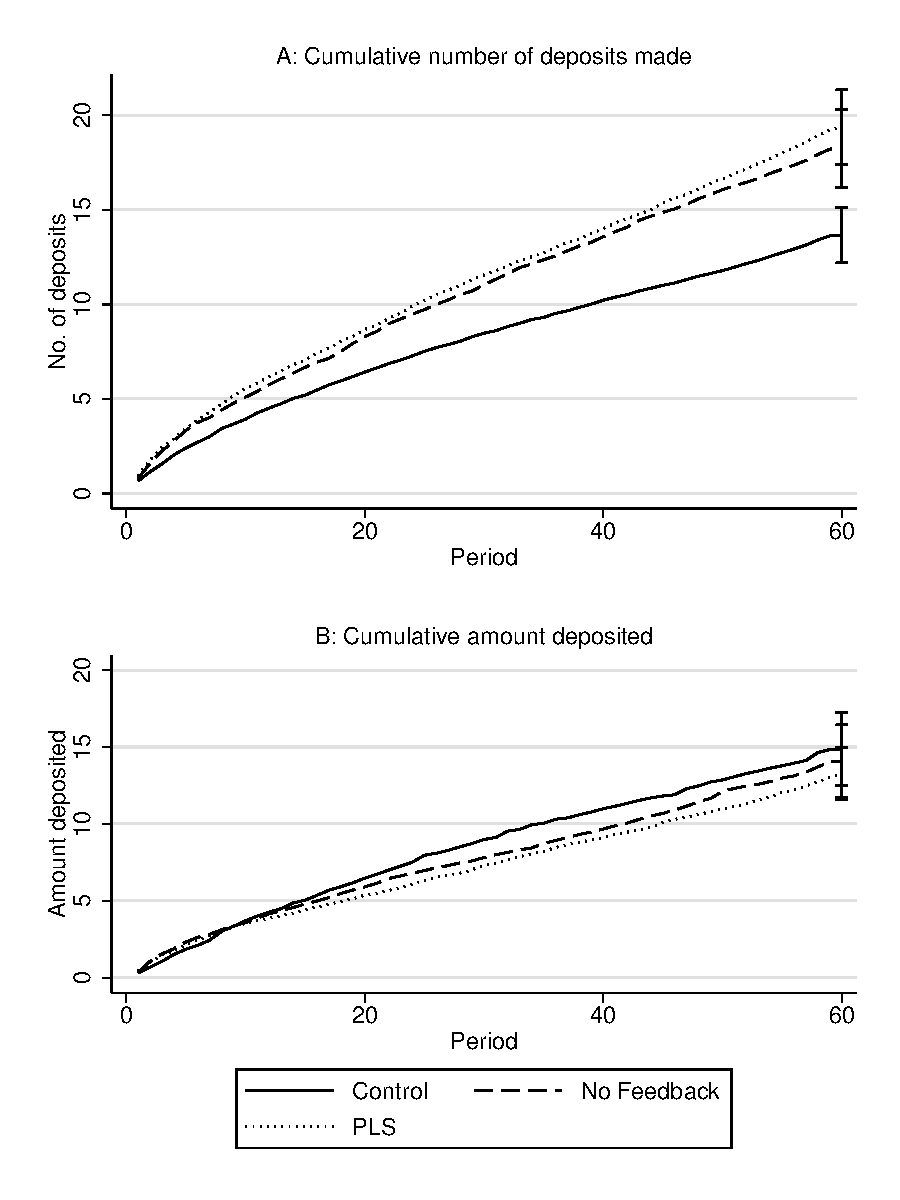
\includegraphics[height=0.85\textheight]{../../figures/line-cumdeposits.pdf}
		\label{fig:line-cumdeposits}
		\caption*{\footnotesize \emph{Notes:} Panel A plots the cumulative number of deposits made by the average participant over the 60-day savings period by treatment assignment. Panel B plots the cumulative amount deposited by the average participant. Error bars for the total number of deposits and total amount deposited by the end of the project are within one standard error of the mean.}
	\end{figure}

	\begin{figure}[h]
	\centering
	\caption{Effects over time -- Number of deposits}
	\centerfloat
	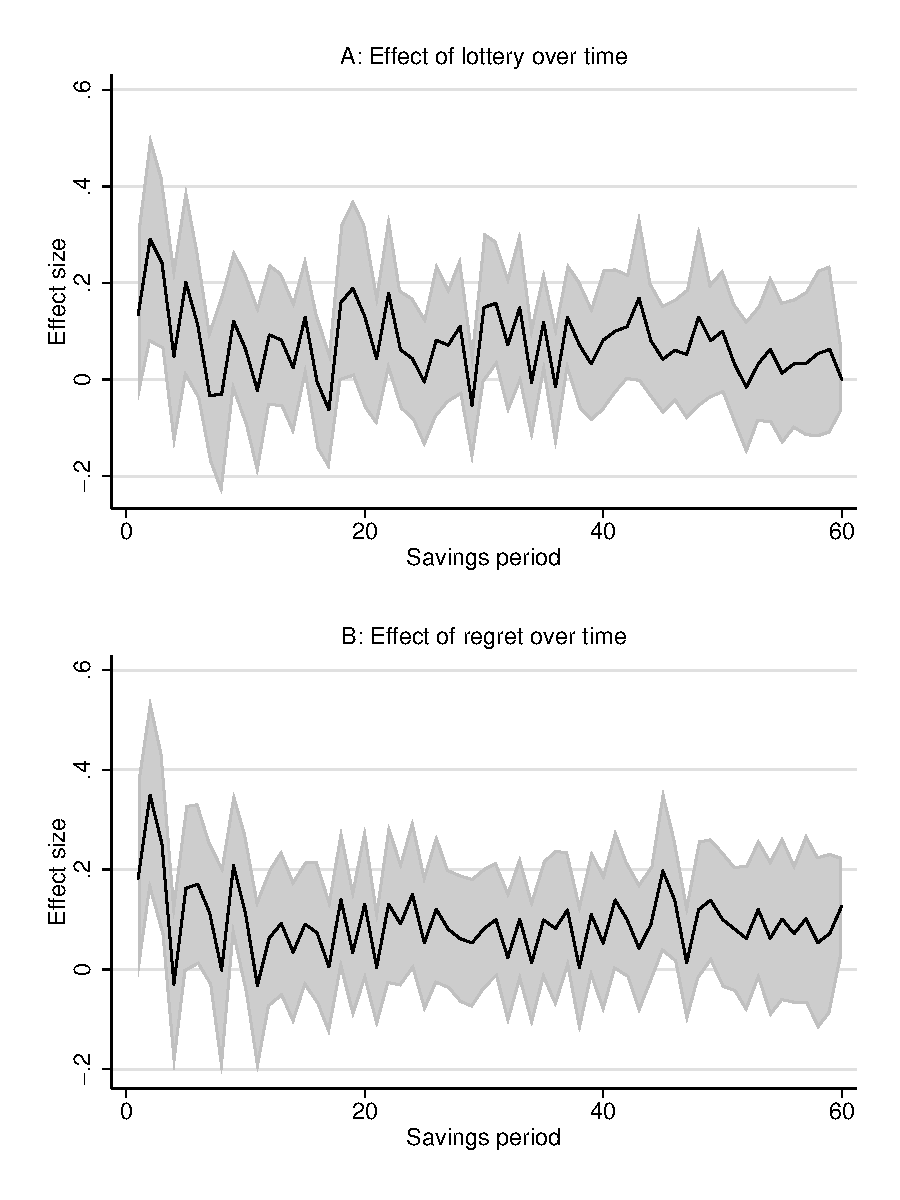
\includegraphics[width=\textwidth]{../../figures/line-timemobile_deposits.pdf}
	\caption*{\footnotesize \emph{Notes:} Panel A plots the treatment effect of \textsc{Lottery} on number of deposits as a function of savings period. Panel B plots the treatment effect of \textsc{Regret} on number of deposits as a function of savings period. Shaded areas represent 95\% confidence regions.}
	\end{figure}

	% \begin{figure}[h]
	% \centering
	% \caption{Effects over time -- Amount deposited}
	% \centerfloat
	% 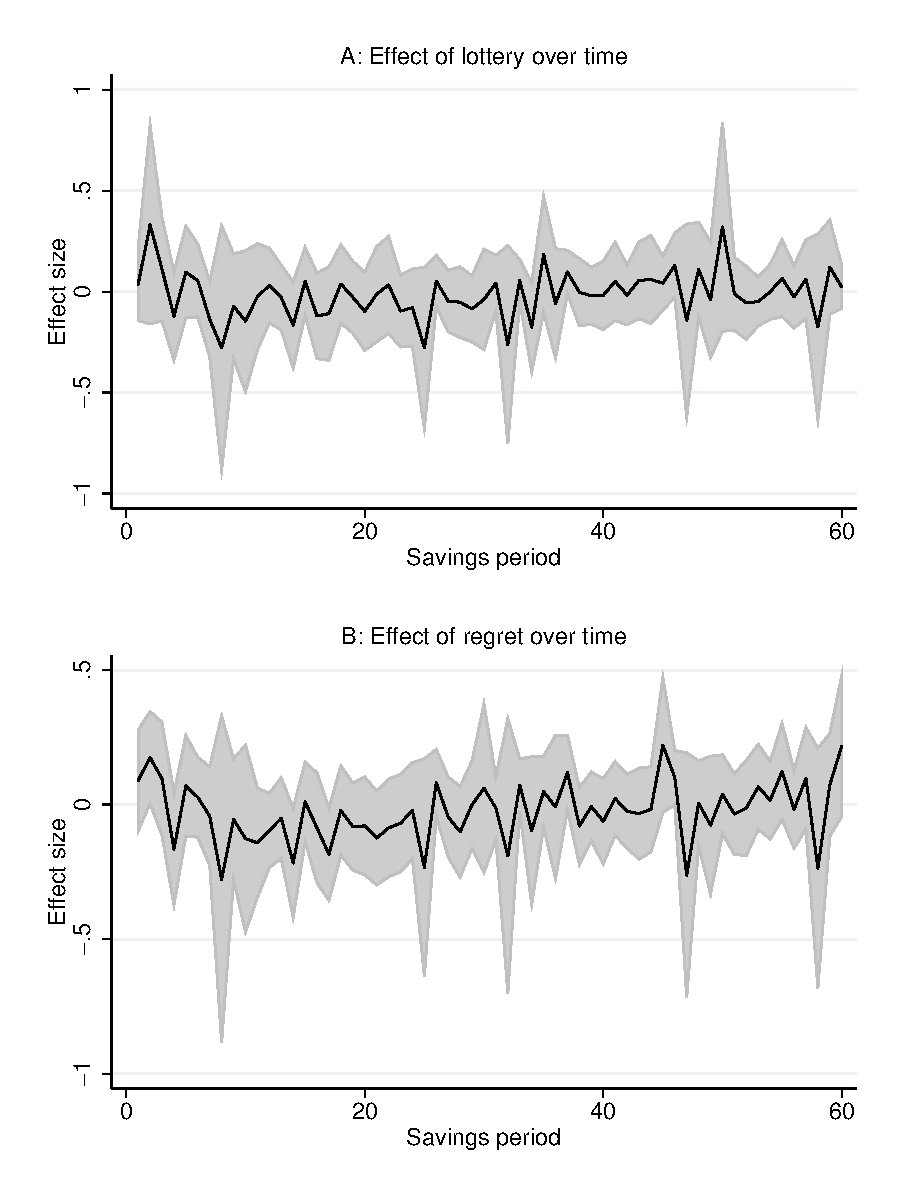
\includegraphics[width=\textwidth]{../../figures/line-timemobile_depositamount.pdf}
	% \caption*{\footnotesize \emph{Notes:} Panel A plots the treatment effect of \textsc{Lottery} on amount deposited as a function of savings period. Panel B plots the treatment effect of \textsc{Regret} on amount deposited as a function of savings period. Shaded areas represent 95\% confidence regions.}
	% \end{figure}

% Notes to self

% Overview of results
%
% 	Regret increases number of deposits (days and not more per day)
% 	Lottery shows some evidence but perhaps underpowered
% 	No effect on balance
% 	Regret increases amount withdrew
% 	Regret increases savings and usage of ROSCA
% 	Regret increases self-reported gambling
% 	Lottery/Regret increases lucky person
% 	Lottery/Regret increases self-selection into regret group
%	Effects on the number of deposits were more acute for participants who are female, who are over 30 years old, with lower incomes, who are less prone to gambling, and who are risk-seeking, though we report no significant heterogeneous effects.

% Possible explanations for results
%
% 	What if these are just the effect of reminders? all groups receive text
% 	Overweighting of probabilities (no because there would have been an effect on amounts)
% 	Fallacy of large numbers (plausible in order to spread risk)
% 	Benartzi Thaler: myopic loss aversion (?)
% 	Liquidity constraints (plausible but check structure of income)
% 	Lumpy gambling utility (plausible but how do we distinguish from others?)
% 	Usage diminishes learning curve, improves trust, etc. (can this be tested?)
% 	Why only ROSCA and not formal savings?
% 	Differences in project period
% 	A possible mechanism underlying this effect could be that participating in the savings lottery affects perceived probabilities of gambling. Recall that our lottery incentive was designed so that savers faced no losses to their deposits. The experience of
% 	Table \ref{tab:reg-self} shows that treated participants rate themselves as being lucky nearly 4.77 - 4.97 SDs ($p < 0.01$) higher than the control group.

% Our contributions
%
% 	First causal evidence of LLDAs on savings and gambling
% 	Developing country setting
% 	Mobile savings allow tight tracking of savings behavior
% 	Multi-period panel setting gives us dynamic information
% 	Test the influence of regret aversion
% 	Focus on a potentially important outcome (no. of deposits/streak) determining long-term savings behavior previously neglected in the literature (Less than 20\% of banked adults in Sub-Saharan Africa make more than 2 deposits in a month \shortcite{demirguc-kunt_global_2015})

% differences with PAP
% think about intertemporal consumer behavior; what does it predict?; what do our results say about the prevailing model?

% no matter how much we dig into panel, a qje paper is not coming out because of our results, more refined story rather than extra analysis
% its promising as a great example of a null result, what are some theories about why this didnt work? i mean its a huge match so we set ourselves up for failure, theres already a ceiling effect
% MA: survey experiment prior duke MBA students get theory from this, lotteries work well when the interest rate is low but not as it increases
% more analysis is good beecause we did everything but always better to have a clear story
% creates participation but welfare impacts are inconclusive
% JPE
% how important to discuss non-sig het effects? at least display the tests for a select number of het effects
% finish reading the Brune paper

\end{document}
